\chapter{Definitions/Notions}
	%%%%%%%%%%%%%%%%%%%%%%%%%%%%%%%%%%%%%%%%%%%%%%%%%%%%%%%%%
	%%%%%%%%%%%%%%%%%%   Architecture   %%%%%%%%%%%%%%%%%%%%%
	%%%%%%%%%%%%%%%%%%%%%%%%%%%%%%%%%%%%%%%%%%%%%%%%%%%%%%%%%
	\section{Architecture}
		The architecture of an IT system is the structure or structures of the system which comprise
		software and hardware components, the externally visible properties of those components,
		and the relationships among them.
		\begin{itemize}
			\item Architecture isn't simply \textit{good} or \textit{bad}
			\item Architectue is fit or unfit \textit{for a purpose}
		\end{itemize}
		\subsection{Goals of an Architecture}
			\begin{itemize}
				\item Producing a framework to support the development of software
				\item Creating an integration platform for future enhancements
				\item Producing the interface definitions for collaboration of components
			\end{itemize}
		\subsection{Importance of Architecture}
			\color{red}\textbf{If the size and complexity of a software system increase, the global structure of the system becomes more important than the selection of specific algorithms and data structures.}\color{black}
		\subsection{Architecture vs. Design}
		An architecture provides a framework and a 'set of rules' for the act of designing a particular thing. So there can be many individually designed instances of each particular architectural style. 
		\subsection{Architecture Levels}
			\subsubsection*{Conceptual Architecture}
				\begin{itemize}
					\item direct attention at an appropriate decomposition of the system without delving into details
					\item  provides a useful vehicle for communicating the architecture to non-technical audiences, such as management, marketing, and users
					\item consists of the Architecture Diagram (without interfaces) and an informal component
					specification for each component (see: ADL)
				\end{itemize}

			
			\subsubsection*{Logical Architecture}
				\begin{itemize}
					\item  adds precision, providing a detailed "blueprint" from which component developers and component users can work in relative independence
					\item  incorporates the detailed Architecture Diagram (with interfaces)
				\end{itemize}
			
			\subsubsection*{Execution/Physical Architecture}
				\begin{itemize}
					\item Shows the mapping of components onto the threads, processes, (virtual) machines, \ldots of the physical system
					\item created for distributed or concurrent systems\Biglb
				\end{itemize}
			
	%%%%%%%%%%%%%%%%%%%%%%%%%%%%%%%%%%%%%%%%%%%%%%%%%%%%%%%%%
	%%%%%%%%%%%%%%%%%%     Architect    %%%%%%%%%%%%%%%%%%%%%
	%%%%%%%%%%%%%%%%%%%%%%%%%%%%%%%%%%%%%%%%%%%%%%%%%%%%%%%%%
	\section{Architect}
		Some interesting definitions/quotations/etc. from various slides\ldots
		\begin{itemize}
			\item The IT Architect defines (i.e. architects) solutions to client business problems through the reasoned application of information technology.
			\item The task of an architect is reduction of complexity to orders of	magnitude that can be realistically handled.
			\item The definition of Vitruvius ($ \approx 25 B.C.$) adds, that an architect (of any kind) should have a lot of general knowledge.
		\end{itemize}
		\red{The architect is the advocate of the client.}
		\subsection{Where do Architects get ideas from?}
			Studies of work of other architects is key!\\
			Importance of reference architectures, patterns, styles\Biglb
		
		\subsection{Architectural thinking}
			Architectural thinking is based on basic architectural principles:
			\begin{itemize}
				\item Separation of concerns
				\item Information Hiding
				\item Design by interface
				\item Separation of interface and implementation
				\item Partitioning/distributing responsibilities
			\end{itemize}
			Architectural thinking involves
			\begin{itemize}
				\item Looking at the solution from the direction of requirements, not technology
				\item Understanding all aspects of the requirements (functional and non-functional)
				\item Understandign all aspects of the solution (functional and non-functional)
				\item Using reference architectures and patterns whenever appropriate
				\item Compromising and balancing; every solution to a requirement will cause other problems
			\end{itemize}
			
			
		
	%%%%%%%%%%%%%%%%%%%%%%%%%%%%%%%%%%%%%%%%%%%%%%%%%%%%%%%%%
	%%%%%%%%%%%%%%%%%%      System     %%%%%%%%%%%%%%%%%%%%%%
	%%%%%%%%%%%%%%%%%%%%%%%%%%%%%%%%%%%%%%%%%%%%%%%%%%%%%%%%%	
	\section{System}
		Composition of parts into a new whole which represents via the collaboration of the parts more than the sum of its parts.
		
		\subsection{Emergence}
		This is a central aspect of Systems: Emergence is the appearance of properties of a system which none
		of its constituents has; i.e. a shelf: it is comprised of wooden planks and screws, and after you finished building it, you can put stuff on it. This is emergence: the planks and screws themselves did not offer the possibility to store things, it emerged from the system that is called \textit{a shelf}.
		
		
	%%%%%%%%%%%%%%%%%%%%%%%%%%%%%%%%%%%%%%%%%%%%%%%%%%%%%%%%%
	%%%%%%%%%%%%%%%%%%       Views      %%%%%%%%%%%%%%%%%%%%%
	%%%%%%%%%%%%%%%%%%%%%%%%%%%%%%%%%%%%%%%%%%%%%%%%%%%%%%%%%	
	\section{Views}
		\begin{itemize}
			\item Views = different models of a single system. Can be built by abstraction
			\item Architecture consists of multiple different model descriptions of a single building. Different model descriptions target different participants (stakeholders) of the project:
		\end{itemize}
		$$ \text{Ground plan} \mapsto \text{Decorator} $$
		$$ \text{Wiring} \mapsto \text{Electrician} $$
		$$ \text{Plumbing} \mapsto \text{Plumber} $$
		$$ \ldots \mapsto \ldots $$
		
		\subsection{Structural and Behavioral Views}
			These are used to enhance understandability of the architecture's levels (see 1.1.4).
			\paragraph*{Structural Views}  consist of the Architecture Diagram, and Component and Interface Specifications

			\paragraph*{Behavioral Views} Contain Component Collaboration or Sequence Diagrams; they answer the question '\textit{How does this work?}'\pagebreak
			
	%%%%%%%%%%%%%%%%%%%%%%%%%%%%%%%%%%%%%%%%%%%%%%%%%%%%%%%%%
	%%%%%%%%%%%%%%%%%%     Together     %%%%%%%%%%%%%%%%%%%%%
	%%%%%%%%%%%%%%%%%%%%%%%%%%%%%%%%%%%%%%%%%%%%%%%%%%%%%%%%%		
	\section{Architectural Levels and Views Together}
		\begin{figure}[h!]
			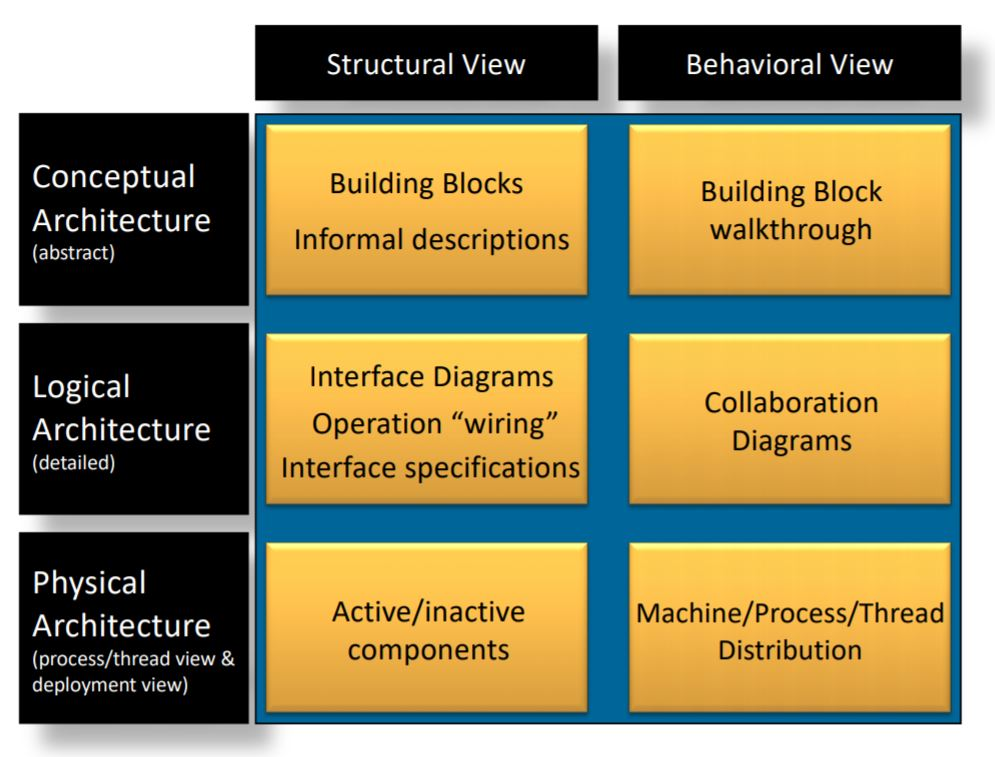
\includegraphics[scale=0.5]{res/arch-levels-and-views.jpg}
		\end{figure}
		

	\section{Reuse}
		\subsection*{Classification}
			\begin{figure}[h!]
				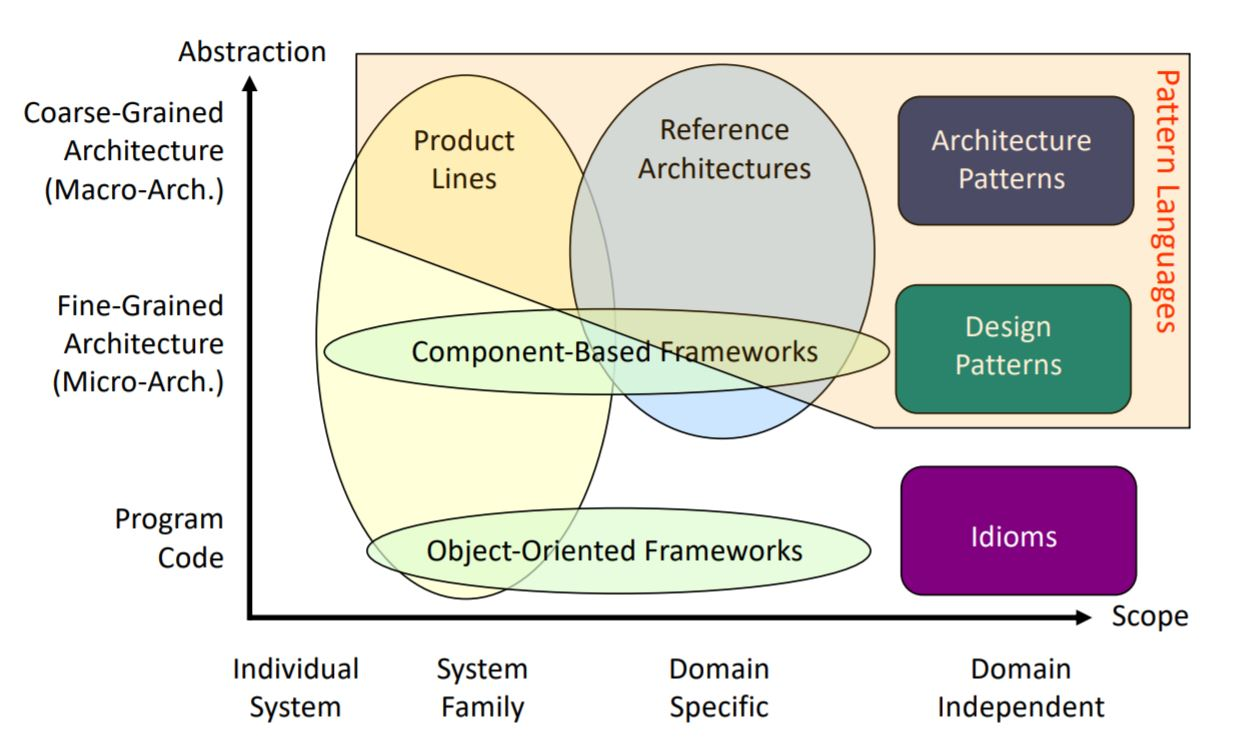
\includegraphics[scale=0.45]{res/reuse-classification.jpg}
			\end{figure}
		
		
		
		
		
	
	
	
	
	
	
	
	
	